\documentclass{article}

\usepackage{graphicx}
\usepackage{tikz}
\usepackage{tikzsymbols}
\usetikzlibrary{calc,patterns,shapes.geometric}
\pagestyle{empty}
\usepackage[margin=0pt]{geometry}
\geometry{papersize={14in,12in}}

\def\centerarc[#1](#2)(#3:#4:#5){\draw[#1] ($(#2)+({#5*cos(#3)},{#5*sin(#3)})$) arc (#3:#4:#5);}

\begin{document}
	\begin{figure}
		\centering
		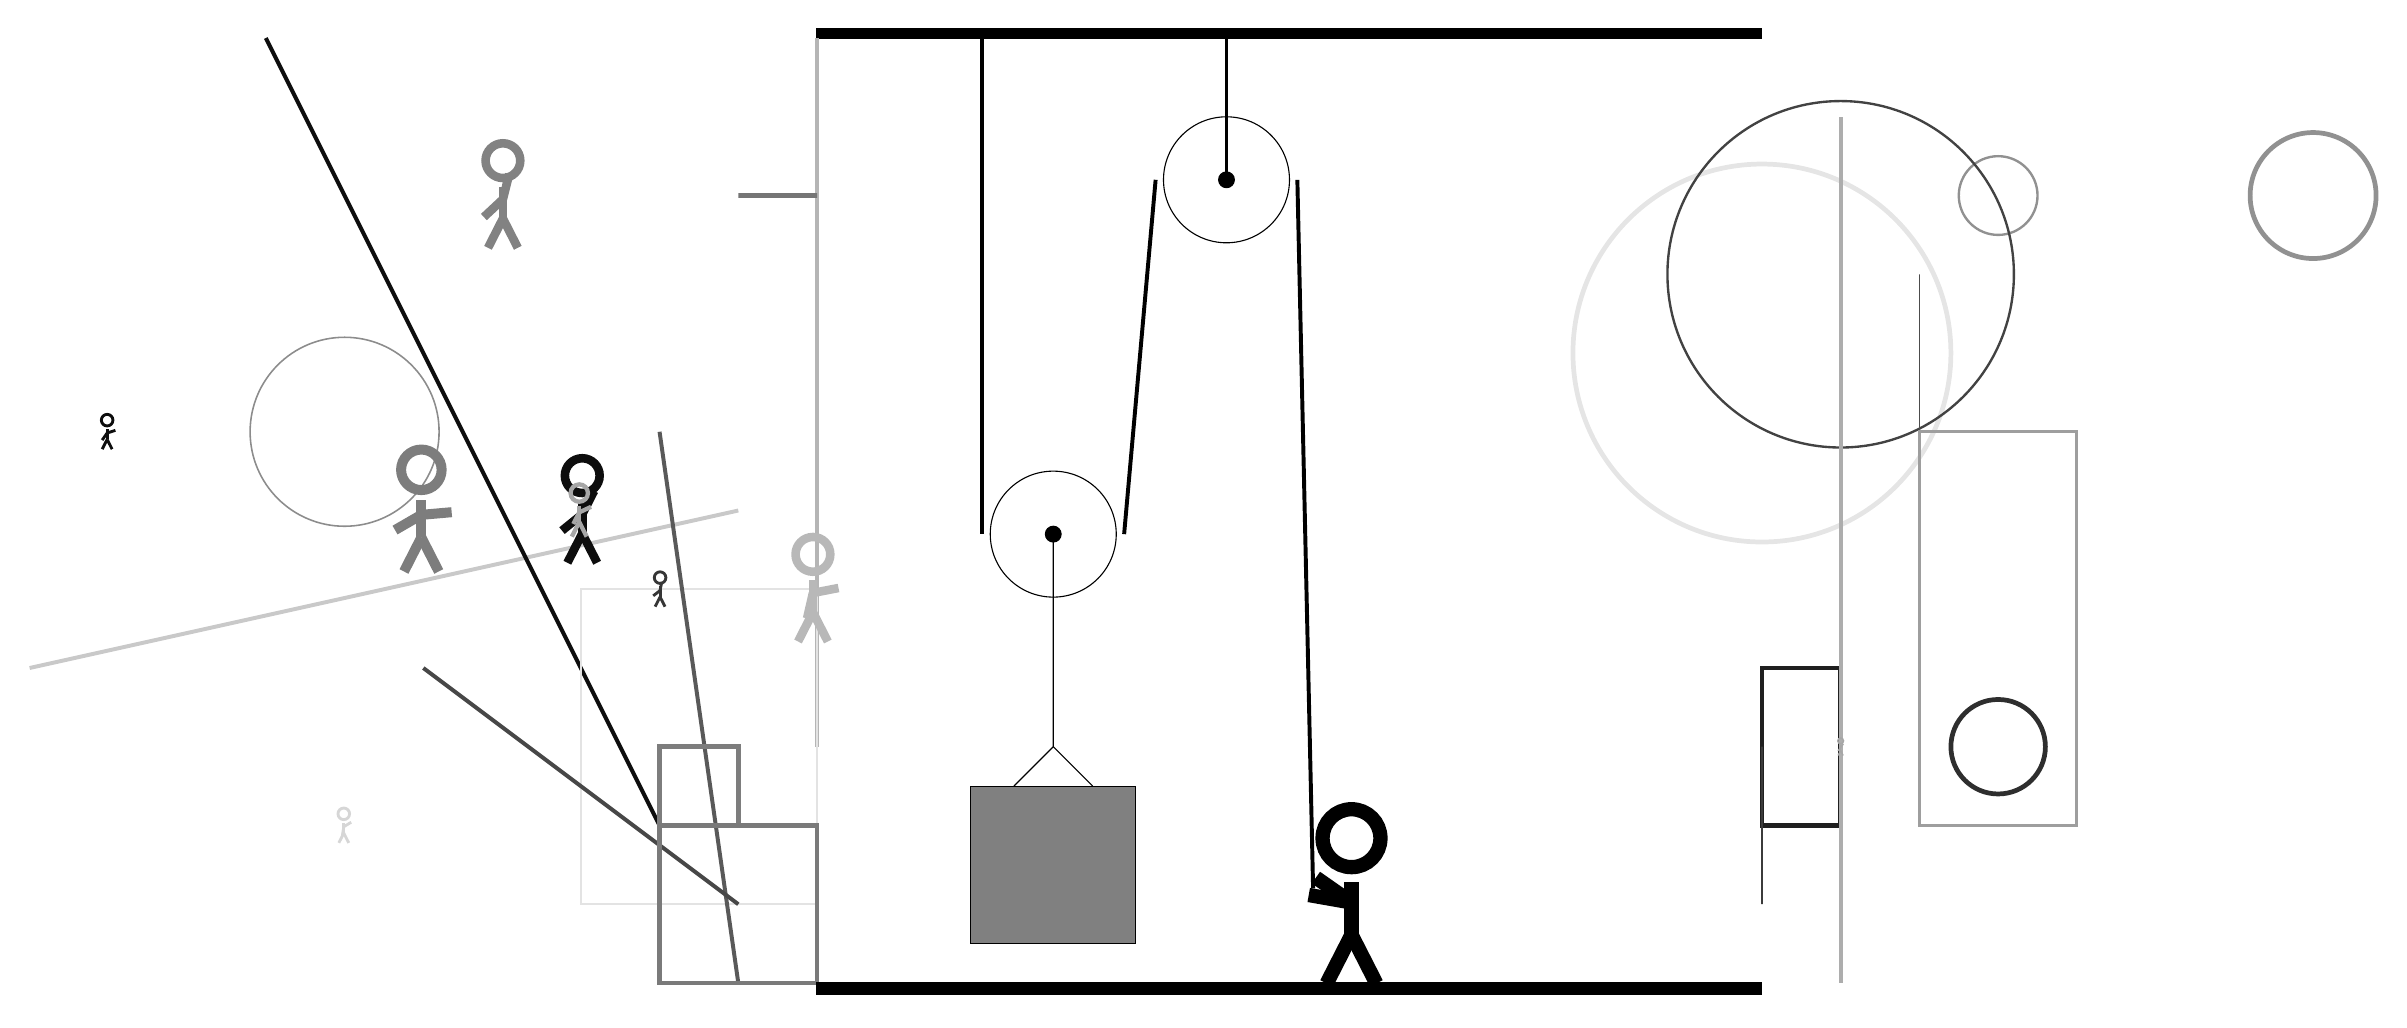
\begin{tikzpicture}
			%%%%% START %%%%%
			
			\draw[fill=black] (-2, 9) rectangle (10, 9.125);
			
			\draw (3.2, 7.2) circle (0.8);
			\draw[fill=black] (3.2, 7.2) circle (0.1);
			\draw[thick] (3.2, 7.2) -- (3.2, 9);
			
			\draw[line width=0.5mm, color=black!58](11, 1) -- (11, -1);
			
			\draw[line width=0.5mm, color=black!21](-3, 3) -- (-12, 1);
			\node[line width=0.7mm, color=black!49] at (-6, 7) {\Strichmaxerl[6][43][76]};
			\node[line width=0.6mm, color=black!95] at (-5, 3) {\Strichmaxerl[6][39][63]};
			\draw [line width=0.2mm, color=black!45](-8, 4) circle (1.2);
			
			\draw [line width=0.6mm, color=black!10](10, 5) circle (2.4);
			
			\draw [line width=0.3mm, color=black!43](13, 7) circle (0.5);
			\draw[line width=0.6mm, color=black!88] (10, -1) rectangle (11, 1);
			\draw[line width=0.5mm, color=black!29](-2, 9) -- (-2, 0);
			\draw[line width=0.6mm, color=black!54] (-3, 7) rectangle (-2, 7);
			\draw[line width=0.2mm, color=black!77] (10, 0) rectangle (10, -2);
			\draw[line width=0.5mm, color=black!95](-4, -1) -- (-9, 9);
			\draw [line width=0.6mm, color=black!43](17, 7) circle (0.8);
			\draw[line width=0.2mm, color=black!11] (-2, -2) rectangle (-5, 2);
			\draw[line width=0.5mm, color=black!65](-4, 4) -- (-3, -3);
			\draw [line width=0.3mm, color=black!74](11, 6) circle (2.2);
			
			\draw[line width=0.5mm, color=black!32](11, -3) -- (11, 8);
			\node[line width=0.5mm, color=black!35] at (11, 0) {\Strichmaxerl[1][53][51]};
			\draw[line width=0.7mm, color=black!51] (-4, -1) rectangle (-3, 0);
			\draw[line width=0.5mm, color=black!72](-3, -2) -- (-7, 1);
			\draw[line width=0.6mm, color=black!52] (-2, -1) rectangle (-4, -3);
			
			\node[line width=0.6mm, color=black!16] at (-8, -1) {\Strichmaxerl[2][81][31]};
			
			\node[line width=0.3mm, color=black!79] at (-4, 2) {\Strichmaxerl[2][38][79]};
			\draw[line width=0.2mm, color=black!70] (12, 1) rectangle (12, 6);
			\node[line width=0.4mm, color=black!28] at (-2, 2) {\Strichmaxerl[6][77][11]};
			\node[line width=0.7mm, color=black!95] at (-11, 4) {\Strichmaxerl[2][55][18]};
			
			\draw[line width=0.4mm, color=black!38] (12, 4) rectangle (14, -1);
			\draw [line width=0.6mm, color=black!82](13, 0) circle (0.6);
			\node[line width=0.3mm, color=black!51] at (-7, 3) {\Strichmaxerl[7][30][5]};
			\node[line width=0.4mm, color=black!35] at (-5, 3) {\Strichmaxerl[3][63][25]};
			
			\draw (1, 2.7) circle (0.8);
			\draw[fill=black] (1, 2.7) circle (0.1);
			
			\draw (1, 2.7) -- (1, 0) -- (0.5, -0.5);
			\draw (1, 0) -- (1.5, -0.5);
			\draw[fill=black!50] (-0.05, -0.5) rectangle (2.05, -2.5);
			
			\draw[line width=0.5mm] (0.1, 9) -- (0.1, 2.7);
			\centerarc[line width=0.5mm](1, 2.7)(180:360:0.9);
			\draw[line width=0.5mm](1.9, 2.7) -- (2.3, 7.2);
			\centerarc[line width=0.5mm](3.2, 7.2)(0:180:0.9);
			\draw[line width=0.5mm](4.1, 7.2) -- (4.3, -1.8);
			
			\node at (4.7, -1.9) {\Strichmaxerl[10][-35][170]};
			
			\draw[fill=black] (-2, -3) rectangle (10, -3.15);
			
			%%%%% END %%%%%
		\end{tikzpicture}
	\end{figure}	
\end{document}